\chapter{Konzept und Theorie}
%Oberflaeche erklären und was passiert

Die Umsetzung des Delay Plugins besteht aus zwei Teilen: Das Delay und die Steuerung der Parameter mit Hilfe einer GUI.

\section{Delay Effekt}

Der Delay Effekt ist im Grunde eine Wiederholung des Eingangsignals zu einer späteren Zeit (siehe \ref{fig:ableton}: Spur 2). Da zu einem späteren Zeitpunkt dieses exakte Signal nicht mehr da ist muss es in einem Buffer gespeichert werden. Zur Vereinfachung wird der Buffer wie ein kreisförmiger Speicher gesehen. Mit Hilfe von dem Modulo-Operator ist dies programmiertechnisch möglich.
Sollte zu einem bestimmten Zeitpunkt das vergangene Signal zum aktuellen Input hinzugefügt werden, so muss eine gewisse Anzahl an Samples im Speicher zurückgesprungen werden. Dies lässt sich mit Hilfe der Samplerate berechnen.
Um dieses Signal nicht nur einmal wiederzugeben sondern langsam abschwächen zu lassen (siehe \ref{fig:ableton}: Spur 3) muss das verzögerte Signal wieder in den Delaybuffer eingespeist werden.

\begin{figure}
	\centering
	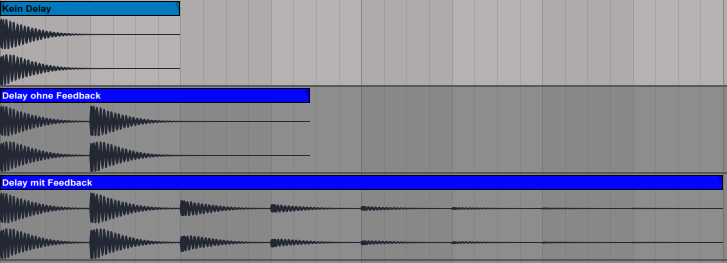
\includegraphics[width=0.8\linewidth]{images/ableton}
	\caption{Ausschnitt aus Ableton Live bei Anwendung des Delay Plugins. 3 verschiedene Audiospuren. 1. Spur: Nur das original Signal. 2. Spur: Signal wird nach 500ms wiederholt. 3. Spur: Wiederholung des Signals mit Einspeisung des verzögerten Signals aber immer leiser werdend. [Siehe Anlage Audio 1 bis 3]}
	\label{fig:ableton}
\end{figure}

Als Veranschaulichung dient hierbei Abbildung \ref{fig:delayline}. Hier werden N Samples direkt vom Input an den Output weitergeleitet als auch im DlyWBuf gespeichert. Das verzögerte Signal \textit{g} wird zusammen mit dem Input addiert und befindet sich dann im Output. \textit{fb} entspricht dem selben Signal wie \textit{g} und wird gleichzeitig mit dem aktuellen Input im Delaybuffer gespeichert.

\begin{figure}
	\centering
	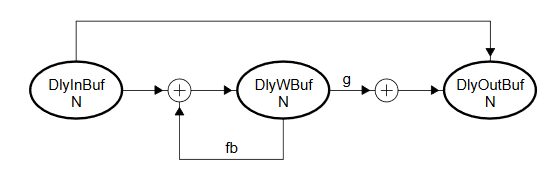
\includegraphics[width=0.7\linewidth]{images/delayline}
	\caption{Ablaufdiagramm einer typischen Delayline mit Feedback. Input landet direkt im Output. Input wird gleichzeitig im Delaybuffer gespeichert. Verzögertes Signal wird zusammen mit Input im Output zusammengeführt. Gleichzeitig wird das verzögerte Signal wieder im Delaybuffer eingespeist. \cite{HTC}}
	\label{fig:delayline}
\end{figure}


\section{GUI}

Es gibt bei dieser Art von Delay 3 Werte die verändert werden könnten. Eine mögliche Umsetzung wäre das Nutzen von 3 Slidern. Einen für den Verzögerungswert (Delaytime), Feedback und Mischverhältnis. Für zukünftige Plugins ist jedoch die Verwendung eines Felds, wo Werte abhängig von einer Position auf der x- und y-Achse sind, von nutzen. 
Slider sind in dem Framework schon standardmäßig dabei, zusammen mit dazugehörigen Observer-Pattern. Zur Anzeige der Werte kann bei dem Slider eine zugehörige TextBox (TextEditor) aktiviert werden.

Das ControlPad muss jedoch selbst umgesetzt werden. Es besteht aus einem Kontrollpunkt (Trackball). Der Mittelpunkt des Trackballs darf nicht das darunterliegende Feld verlassen. Um die Werte anzuzeigen, welche die jeweilige Achsenposition repräsentieren, gibt es noch zwei TextBoxen (xValue, yValue). Alles zusammen ergibt das Element \textit{ControlPad }.

Das Hintergrundbild wirkt als Anlehnung an das Echo in den Bergen. 

\begin{figure}
	\centering
	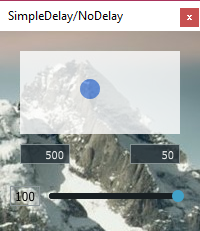
\includegraphics[width=0.5\linewidth]{images/plugininableton}
	\caption{}
	\label{fig:plugininableton}
\end{figure}


